% =============================================================================
\section{Tu primer reto: la estrella del show}
% =============================================================================

\begin{frame}{La misión}
  \begin{columns}[c]
    \column{0.58\textwidth}\centering
    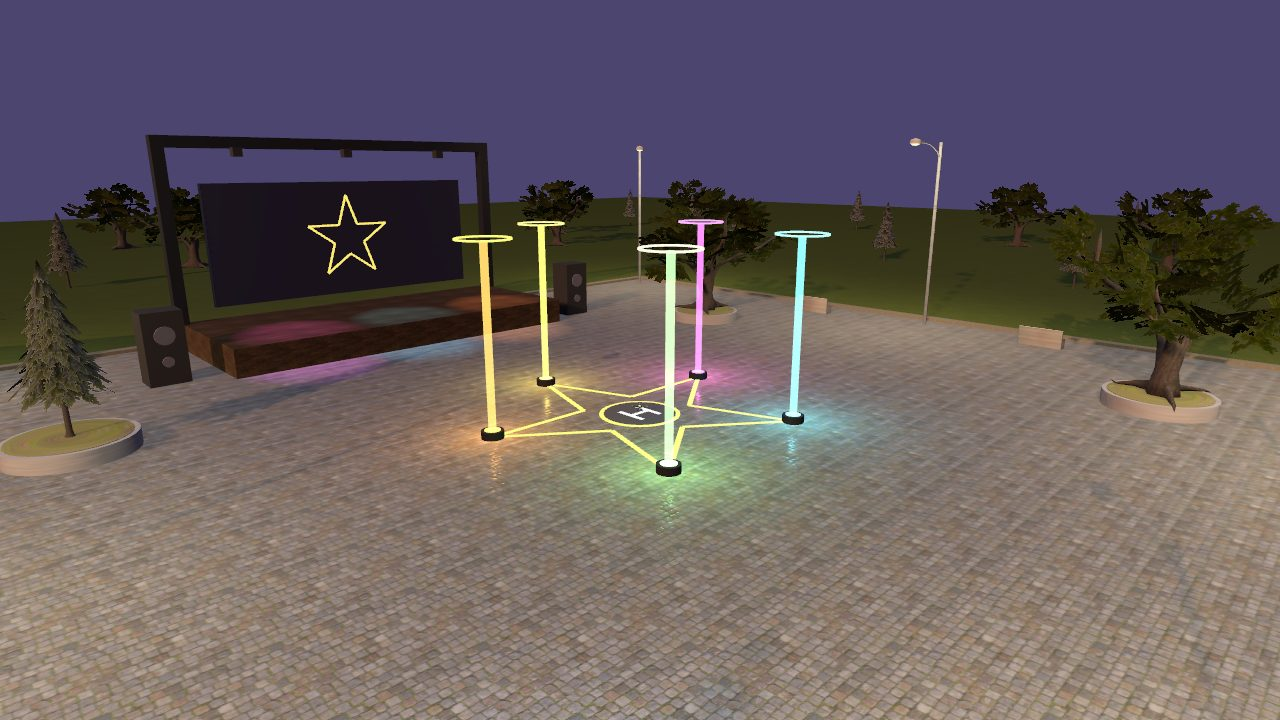
\includegraphics[width=\linewidth]{plaza_show_estrella}\\
    \credito{El mundo \cmd{plaza\_show} de \cmd{x500\_retos} (render propio)}
    \column{0.39\textwidth}\small
    Año nuevo en la plaza. El dron tiene que \textbf{dibujar una estrella en el cielo} pasando por los aros de
    luz.
    \begin{itemize}
      \item Mundo: \cmd{plaza\_show}.
      \item Nodo: \cmd{estrella\_show}, de \cmd{x500\_retos}.
      \item Viene de \cmd{square\_mission} (waypoints en offboard) y \cmd{orbit\_mission} (parámetros).
      \item \textbf{Lo nuevo}: los waypoints ya no se escriben a mano, se \textbf{calculan con una fórmula}.
    \end{itemize}
  \end{columns}
\end{frame}

\begin{frame}{Qué ya está hecho y qué te toca}
  \centering
  \begin{tikzpicture}[every node/.style={font=\scriptsize,align=center},
      es/.style={draw=verde,fill=verdeclaro,rounded corners,minimum width=1.75cm,minimum height=0.9cm}]
    \node[es] (w) at (0,0) {WARMUP};
    \node[es] (t) at (2.3,0) {TAKEOFF};
    \node[es] (s) at (4.6,0) {STAR};
    \node[es] (c) at (6.9,0) {CENTER};
    \node[es] (l) at (9.2,0) {LANDING};
    \node[es] (d) at (11.5,0) {DONE};
    \foreach \a/\b in {w/t,t/s,s/c,c/l,l/d} \draw[-{Stealth},thick] (\a) -- (\b);
    \node[draw=rojo,fill=red!8,rounded corners,line width=1pt,minimum width=3.2cm,minimum height=1cm] (v) at (4.6,-2.0)
      {\cmd{vertices()}\\\textbf{TODO 1 y 2}: \color{rojo}tu parte};
    \draw[-{Stealth},thick,rojo] (v) -- node[right,font=\tiny]{la lista de puntos} (s);
  \end{tikzpicture}
  \vspace{0.6em}

  \raggedright\small
  \begin{itemize}
    \item En \textcolor{verde}{verde}: ya funciona. Despega, recorre la lista, regresa al centro, aterriza y te
      dice qué tan bien lo hiciste.
    \item En \textcolor{rojo}{rojo}: \cmd{vertices()} regresa la lista de puntos de la estrella. Hoy regresa una
      lista \textbf{vacía}.
    \item Si lo corres sin hacer nada, despega, te avisa y aterriza:
  \end{itemize}
  \begin{terminal}{ros2 run x500\_retos estrella\_show}
vertices() regresó una lista vacía: falta el TODO. Aterrizando
  \end{terminal}
\end{frame}

\begin{frame}{La geometría, paso a paso}
  \begin{columns}[c]
    \column{0.47\textwidth}\centering
    \begin{tikzpicture}[scale=0.62]
      \draw[gray!20,step=1] (-5.6,-5.6) grid (5.6,5.6);
      \draw[-{Stealth},verde,thick] (0,-5.6) -- (0,5.9) node[above,font=\tiny] {N};
      \draw[-{Stealth},rojo,thick] (-5.6,0) -- (5.9,0) node[right,font=\tiny] {E};
      \draw[azul!50,thick] (0,0) circle (5);
      \draw[|-|,gris,visible on=<1>] (0,0) -- (-5,0) node[midway,below,font=\tiny] {R = radius};
      \draw[naranja!60,thick,visible on=<3->] (0,0) circle (1.91);
      % picos: ángulo 72k desde el norte hacia el este -> (E, N) = (R sen a, R cos a)
      \foreach \k in {0,...,4} {
        \pgfmathsetmacro{\a}{72*\k}
        \pgfmathtruncatemacro{\pp}{\k==0 ? 1 : 2}
        \pgfmathtruncatemacro{\ii}{\k==0 ? 3 : 4}
        \fill[azul,visible on=<\pp->] ({5*sin(\a)},{5*cos(\a)}) circle (4.5pt);
        \node[font=\tiny\bfseries,visible on=<\pp->] at ({5.7*sin(\a)},{5.7*cos(\a)}) {P\k};
        \pgfmathsetmacro{\b}{72*\k+36}
        \fill[naranja,visible on=<\ii->] ({1.91*sin(\b)},{1.91*cos(\b)}) circle (4pt);
        \node[font=\tiny\bfseries,visible on=<\ii->] at ({2.55*sin(\b)},{2.55*cos(\b)}) {I\k};
      }
      \draw[gris,visible on=<2>] (0,1.2) arc (90:18:1.2) node[midway,above right,font=\tiny] {72°};
      \draw[azul,line width=1.5pt,visible on=<5->,-{Stealth}]
        plot coordinates {(0,5) ({1.91*sin(36)},{1.91*cos(36)}) ({5*sin(72)},{5*cos(72)}) ({1.91*sin(108)},{1.91*cos(108)})
          ({5*sin(144)},{5*cos(144)}) ({1.91*sin(180)},{1.91*cos(180)}) ({5*sin(216)},{5*cos(216)})
          ({1.91*sin(252)},{1.91*cos(252)}) ({5*sin(288)},{5*cos(288)}) ({1.91*sin(324)},{1.91*cos(324)}) (0,5)};
      \only<5>{\node at (0,5) {\dronarriba{0.8cm}};}
    \end{tikzpicture}
    \column{0.5\textwidth}\small
    \only<1>{\textbf{1. El círculo.} Todos los picos están en un círculo de radio \cmd{radius} (5 m). El primero,
      \textbf{P0}, al norte.}%
    \only<2>{\textbf{2. Los picos.} Con \cmd{points} = 5 picos, entre uno y otro hay $360°/5 = 72°$. El pico
      $k$ está a un ángulo $\frac{2\pi k}{\text{points}}$ (en radianes) medido desde el norte hacia el este.
      \textbf{Esto es el TODO 1.}}%
    \only<3>{\textbf{3. El círculo de adentro.} Los vértices interiores están en un círculo más chico: radio
      \cmd{radius * inner\_ratio} ($5 \times 0.382 = 1.91$ m). \textbf{I0} va a la mitad, en ángulo, entre P0 y
      P1.}%
    \only<4>{\textbf{4. Todos los interiores.} Uno después de cada pico. \textbf{Esto es el TODO 2.} Si
      \cmd{inner\_ratio} es 0, no hay interiores.}%
    \only<5>{\textbf{5. El orden de vuelo.} P0, I0, P1, I1, \ldots, P4, I4 y de vuelta. Esa es la lista que
      \cmd{vertices()} tiene que regresar; el resto del nodo la vuela.}%
  \end{columns}
\end{frame}

\begin{frame}{De ángulo a norte y este}
  \begin{columns}[c]
    \column{0.42\textwidth}\centering
    \begin{tikzpicture}[scale=1.1]
      \draw[-{Stealth},verde,thick] (0,0) -- (0,2.7) node[above,font=\tiny] {Norte};
      \draw[-{Stealth},rojo,thick] (0,0) -- (2.7,0) node[right,font=\tiny] {Este};
      \draw[azul,thick] (0,0) -- (1.5,2.0);
      \fill[azul] (1.5,2.0) circle (2.5pt) node[above right,font=\tiny] {punto};
      \draw[dashed,gray] (1.5,2.0) -- (1.5,0) node[below,font=\tiny] {$r\sin a$};
      \draw[dashed,gray] (1.5,2.0) -- (0,2.0) node[left,font=\tiny] {$r\cos a$};
      \draw (0,0.7) arc (90:53:0.7); \node[font=\tiny] at (0.3,0.95) {$a$};
      \node[font=\tiny,azul] at (0.55,1.25) {$r$};
    \end{tikzpicture}
    \column{0.55\textwidth}\small
    Un punto a distancia $r$ y ángulo $a$ (desde el norte, girando hacia el este):
    \[ \text{norte} = r\cos a \qquad \text{este} = r\sin a \]
    En el código, cada vértice es \cmd{\{norte, este, z\}} con \cmd{z = -altitude} y se agrega con
    \cmd{out.push\_back(\{norte, este, z\});}
    \begin{ojo}
      \small
      \begin{itemize}
        \item \cmd{std::cos} y \cmd{std::sin} usan \textbf{radianes}, no grados.
        \item \cmd{k / points\_} con dos enteros da \textbf{0}: multiplica primero por \cmd{2 * M\_PI}.
        \item \cmd{radius\_} es \cmd{double} y el punto lleva \cmd{float}: \cmd{static\_cast<float>(...)}.
      \end{itemize}
    \end{ojo}
  \end{columns}
\end{frame}

\begin{frame}[fragile]{Pruébalo}
  \begin{lstlisting}[style=bash]
vespo up --sim --world plaza_show                     # terminal 1
ros2 run x500_retos estrella_show                     # terminal 2
# ... cambias vertices() en src/x500_retos/src/estrella_show.cpp ...
vespo build x500_retos                                # y otra vez ros2 run
  \end{lstlisting}
  \begin{columns}[c]
    \column{0.5\textwidth}
    \begin{terminal}{al final, si salió bien}
Aterrizado. Qué tan cerca pasó de cada vértice:\\
\ \ \ 1: 0.08 m OK\\
\ \ \ 2: 0.11 m OK\\
\ \ \ \ldots\\
\ \ 10: 0.09 m OK\\
Misión cumplida
    \end{terminal}
    \column{0.47\textwidth}\small
    \textbf{Se cumple si} pasa a menos de \textbf{0.5 m} de cada vértice, regresa al centro y aterriza. Si uno dice
    \textcolor{rojo}{FALLÓ}, ese punto quedó mal calculado.
  \end{columns}
\end{frame}

\begin{frame}[fragile]{Si tu fórmula es correcta, sirve para todo}
  \begin{columns}[t]
    \column{0.32\textwidth}\centering
    \begin{tikzpicture}[scale=0.32]
      \draw[azul,line width=1.2pt] plot coordinates {(0,5) ({1.91*sin(36)},{1.91*cos(36)}) ({5*sin(72)},{5*cos(72)}) ({1.91*sin(108)},{1.91*cos(108)})
          ({5*sin(144)},{5*cos(144)}) ({1.91*sin(180)},{1.91*cos(180)}) ({5*sin(216)},{5*cos(216)})
          ({1.91*sin(252)},{1.91*cos(252)}) ({5*sin(288)},{5*cos(288)}) ({1.91*sin(324)},{1.91*cos(324)}) (0,5)};
    \end{tikzpicture}\\
    \scriptsize por defecto\\\cmd{points:=5}
    \column{0.32\textwidth}\centering
    \begin{tikzpicture}[scale=0.32]
      \draw[azul,line width=1.2pt] plot coordinates {(0,5) ({2.5*sin(30)},{2.5*cos(30)}) ({5*sin(60)},{5*cos(60)}) ({2.5*sin(90)},{2.5*cos(90)})
          ({5*sin(120)},{5*cos(120)}) ({2.5*sin(150)},{2.5*cos(150)}) ({5*sin(180)},{5*cos(180)}) ({2.5*sin(210)},{2.5*cos(210)})
          ({5*sin(240)},{5*cos(240)}) ({2.5*sin(270)},{2.5*cos(270)}) ({5*sin(300)},{5*cos(300)}) ({2.5*sin(330)},{2.5*cos(330)}) (0,5)};
    \end{tikzpicture}\\
    \scriptsize\cmd{points:=6}\\\cmd{inner\_ratio:=0.5}
    \column{0.32\textwidth}\centering
    \begin{tikzpicture}[scale=0.32]
      \draw[azul,line width=1.2pt] (0,5) -- (5,0) -- (0,-5) -- (-5,0) -- cycle;
    \end{tikzpicture}\\
    \scriptsize\cmd{points:=4}\\\cmd{inner\_ratio:=0.0}: ¡un cuadrado!
  \end{columns}
  \vspace{0.4em}
  \begin{lstlisting}[style=bash]
ros2 run x500_retos estrella_show --ros-args -p points:=6 -p inner_ratio:=0.5
ros2 run x500_retos estrella_show --ros-args -p points:=4 -p inner_ratio:=0.0
  \end{lstlisting}
  \small Con 4 picos y sin interiores es el \cmd{square\_mission}, pero calculado: el mismo código hace las tres
  figuras.
\end{frame}
